% Options for packages loaded elsewhere
\PassOptionsToPackage{unicode}{hyperref}
\PassOptionsToPackage{hyphens}{url}
\PassOptionsToPackage{dvipsnames,svgnames,x11names}{xcolor}
%
\documentclass[
  letterpaper,
  DIV=11,
  numbers=noendperiod]{scrartcl}

\usepackage{amsmath,amssymb}
\usepackage{iftex}
\ifPDFTeX
  \usepackage[T1]{fontenc}
  \usepackage[utf8]{inputenc}
  \usepackage{textcomp} % provide euro and other symbols
\else % if luatex or xetex
  \usepackage{unicode-math}
  \defaultfontfeatures{Scale=MatchLowercase}
  \defaultfontfeatures[\rmfamily]{Ligatures=TeX,Scale=1}
\fi
\usepackage{lmodern}
\ifPDFTeX\else  
    % xetex/luatex font selection
\fi
% Use upquote if available, for straight quotes in verbatim environments
\IfFileExists{upquote.sty}{\usepackage{upquote}}{}
\IfFileExists{microtype.sty}{% use microtype if available
  \usepackage[]{microtype}
  \UseMicrotypeSet[protrusion]{basicmath} % disable protrusion for tt fonts
}{}
\makeatletter
\@ifundefined{KOMAClassName}{% if non-KOMA class
  \IfFileExists{parskip.sty}{%
    \usepackage{parskip}
  }{% else
    \setlength{\parindent}{0pt}
    \setlength{\parskip}{6pt plus 2pt minus 1pt}}
}{% if KOMA class
  \KOMAoptions{parskip=half}}
\makeatother
\usepackage{xcolor}
\setlength{\emergencystretch}{3em} % prevent overfull lines
\setcounter{secnumdepth}{-\maxdimen} % remove section numbering
% Make \paragraph and \subparagraph free-standing
\ifx\paragraph\undefined\else
  \let\oldparagraph\paragraph
  \renewcommand{\paragraph}[1]{\oldparagraph{#1}\mbox{}}
\fi
\ifx\subparagraph\undefined\else
  \let\oldsubparagraph\subparagraph
  \renewcommand{\subparagraph}[1]{\oldsubparagraph{#1}\mbox{}}
\fi

\usepackage{color}
\usepackage{fancyvrb}
\newcommand{\VerbBar}{|}
\newcommand{\VERB}{\Verb[commandchars=\\\{\}]}
\DefineVerbatimEnvironment{Highlighting}{Verbatim}{commandchars=\\\{\}}
% Add ',fontsize=\small' for more characters per line
\usepackage{framed}
\definecolor{shadecolor}{RGB}{241,243,245}
\newenvironment{Shaded}{\begin{snugshade}}{\end{snugshade}}
\newcommand{\AlertTok}[1]{\textcolor[rgb]{0.68,0.00,0.00}{#1}}
\newcommand{\AnnotationTok}[1]{\textcolor[rgb]{0.37,0.37,0.37}{#1}}
\newcommand{\AttributeTok}[1]{\textcolor[rgb]{0.40,0.45,0.13}{#1}}
\newcommand{\BaseNTok}[1]{\textcolor[rgb]{0.68,0.00,0.00}{#1}}
\newcommand{\BuiltInTok}[1]{\textcolor[rgb]{0.00,0.23,0.31}{#1}}
\newcommand{\CharTok}[1]{\textcolor[rgb]{0.13,0.47,0.30}{#1}}
\newcommand{\CommentTok}[1]{\textcolor[rgb]{0.37,0.37,0.37}{#1}}
\newcommand{\CommentVarTok}[1]{\textcolor[rgb]{0.37,0.37,0.37}{\textit{#1}}}
\newcommand{\ConstantTok}[1]{\textcolor[rgb]{0.56,0.35,0.01}{#1}}
\newcommand{\ControlFlowTok}[1]{\textcolor[rgb]{0.00,0.23,0.31}{#1}}
\newcommand{\DataTypeTok}[1]{\textcolor[rgb]{0.68,0.00,0.00}{#1}}
\newcommand{\DecValTok}[1]{\textcolor[rgb]{0.68,0.00,0.00}{#1}}
\newcommand{\DocumentationTok}[1]{\textcolor[rgb]{0.37,0.37,0.37}{\textit{#1}}}
\newcommand{\ErrorTok}[1]{\textcolor[rgb]{0.68,0.00,0.00}{#1}}
\newcommand{\ExtensionTok}[1]{\textcolor[rgb]{0.00,0.23,0.31}{#1}}
\newcommand{\FloatTok}[1]{\textcolor[rgb]{0.68,0.00,0.00}{#1}}
\newcommand{\FunctionTok}[1]{\textcolor[rgb]{0.28,0.35,0.67}{#1}}
\newcommand{\ImportTok}[1]{\textcolor[rgb]{0.00,0.46,0.62}{#1}}
\newcommand{\InformationTok}[1]{\textcolor[rgb]{0.37,0.37,0.37}{#1}}
\newcommand{\KeywordTok}[1]{\textcolor[rgb]{0.00,0.23,0.31}{#1}}
\newcommand{\NormalTok}[1]{\textcolor[rgb]{0.00,0.23,0.31}{#1}}
\newcommand{\OperatorTok}[1]{\textcolor[rgb]{0.37,0.37,0.37}{#1}}
\newcommand{\OtherTok}[1]{\textcolor[rgb]{0.00,0.23,0.31}{#1}}
\newcommand{\PreprocessorTok}[1]{\textcolor[rgb]{0.68,0.00,0.00}{#1}}
\newcommand{\RegionMarkerTok}[1]{\textcolor[rgb]{0.00,0.23,0.31}{#1}}
\newcommand{\SpecialCharTok}[1]{\textcolor[rgb]{0.37,0.37,0.37}{#1}}
\newcommand{\SpecialStringTok}[1]{\textcolor[rgb]{0.13,0.47,0.30}{#1}}
\newcommand{\StringTok}[1]{\textcolor[rgb]{0.13,0.47,0.30}{#1}}
\newcommand{\VariableTok}[1]{\textcolor[rgb]{0.07,0.07,0.07}{#1}}
\newcommand{\VerbatimStringTok}[1]{\textcolor[rgb]{0.13,0.47,0.30}{#1}}
\newcommand{\WarningTok}[1]{\textcolor[rgb]{0.37,0.37,0.37}{\textit{#1}}}

\providecommand{\tightlist}{%
  \setlength{\itemsep}{0pt}\setlength{\parskip}{0pt}}\usepackage{longtable,booktabs,array}
\usepackage{calc} % for calculating minipage widths
% Correct order of tables after \paragraph or \subparagraph
\usepackage{etoolbox}
\makeatletter
\patchcmd\longtable{\par}{\if@noskipsec\mbox{}\fi\par}{}{}
\makeatother
% Allow footnotes in longtable head/foot
\IfFileExists{footnotehyper.sty}{\usepackage{footnotehyper}}{\usepackage{footnote}}
\makesavenoteenv{longtable}
\usepackage{graphicx}
\makeatletter
\def\maxwidth{\ifdim\Gin@nat@width>\linewidth\linewidth\else\Gin@nat@width\fi}
\def\maxheight{\ifdim\Gin@nat@height>\textheight\textheight\else\Gin@nat@height\fi}
\makeatother
% Scale images if necessary, so that they will not overflow the page
% margins by default, and it is still possible to overwrite the defaults
% using explicit options in \includegraphics[width, height, ...]{}
\setkeys{Gin}{width=\maxwidth,height=\maxheight,keepaspectratio}
% Set default figure placement to htbp
\makeatletter
\def\fps@figure{htbp}
\makeatother

\KOMAoption{captions}{tableheading}
\makeatletter
\@ifpackageloaded{caption}{}{\usepackage{caption}}
\AtBeginDocument{%
\ifdefined\contentsname
  \renewcommand*\contentsname{Table of contents}
\else
  \newcommand\contentsname{Table of contents}
\fi
\ifdefined\listfigurename
  \renewcommand*\listfigurename{List of Figures}
\else
  \newcommand\listfigurename{List of Figures}
\fi
\ifdefined\listtablename
  \renewcommand*\listtablename{List of Tables}
\else
  \newcommand\listtablename{List of Tables}
\fi
\ifdefined\figurename
  \renewcommand*\figurename{Figure}
\else
  \newcommand\figurename{Figure}
\fi
\ifdefined\tablename
  \renewcommand*\tablename{Table}
\else
  \newcommand\tablename{Table}
\fi
}
\@ifpackageloaded{float}{}{\usepackage{float}}
\floatstyle{ruled}
\@ifundefined{c@chapter}{\newfloat{codelisting}{h}{lop}}{\newfloat{codelisting}{h}{lop}[chapter]}
\floatname{codelisting}{Listing}
\newcommand*\listoflistings{\listof{codelisting}{List of Listings}}
\makeatother
\makeatletter
\makeatother
\makeatletter
\@ifpackageloaded{caption}{}{\usepackage{caption}}
\@ifpackageloaded{subcaption}{}{\usepackage{subcaption}}
\makeatother
\ifLuaTeX
  \usepackage{selnolig}  % disable illegal ligatures
\fi
\usepackage{bookmark}

\IfFileExists{xurl.sty}{\usepackage{xurl}}{} % add URL line breaks if available
\urlstyle{same} % disable monospaced font for URLs
\hypersetup{
  colorlinks=true,
  linkcolor={blue},
  filecolor={Maroon},
  citecolor={Blue},
  urlcolor={Blue},
  pdfcreator={LaTeX via pandoc}}

\author{}
\date{}

\begin{document}

\section*{Dynamic Problem Statement}\label{dynamic-problem-statement}
\addcontentsline{toc}{section}{Dynamic Problem Statement}

This is a dynamic rendering of the problem with dynamic variables based
on the username entered.

\subsection{Problem Image}\label{problem-image}

\begin{figure}[H]

{\centering 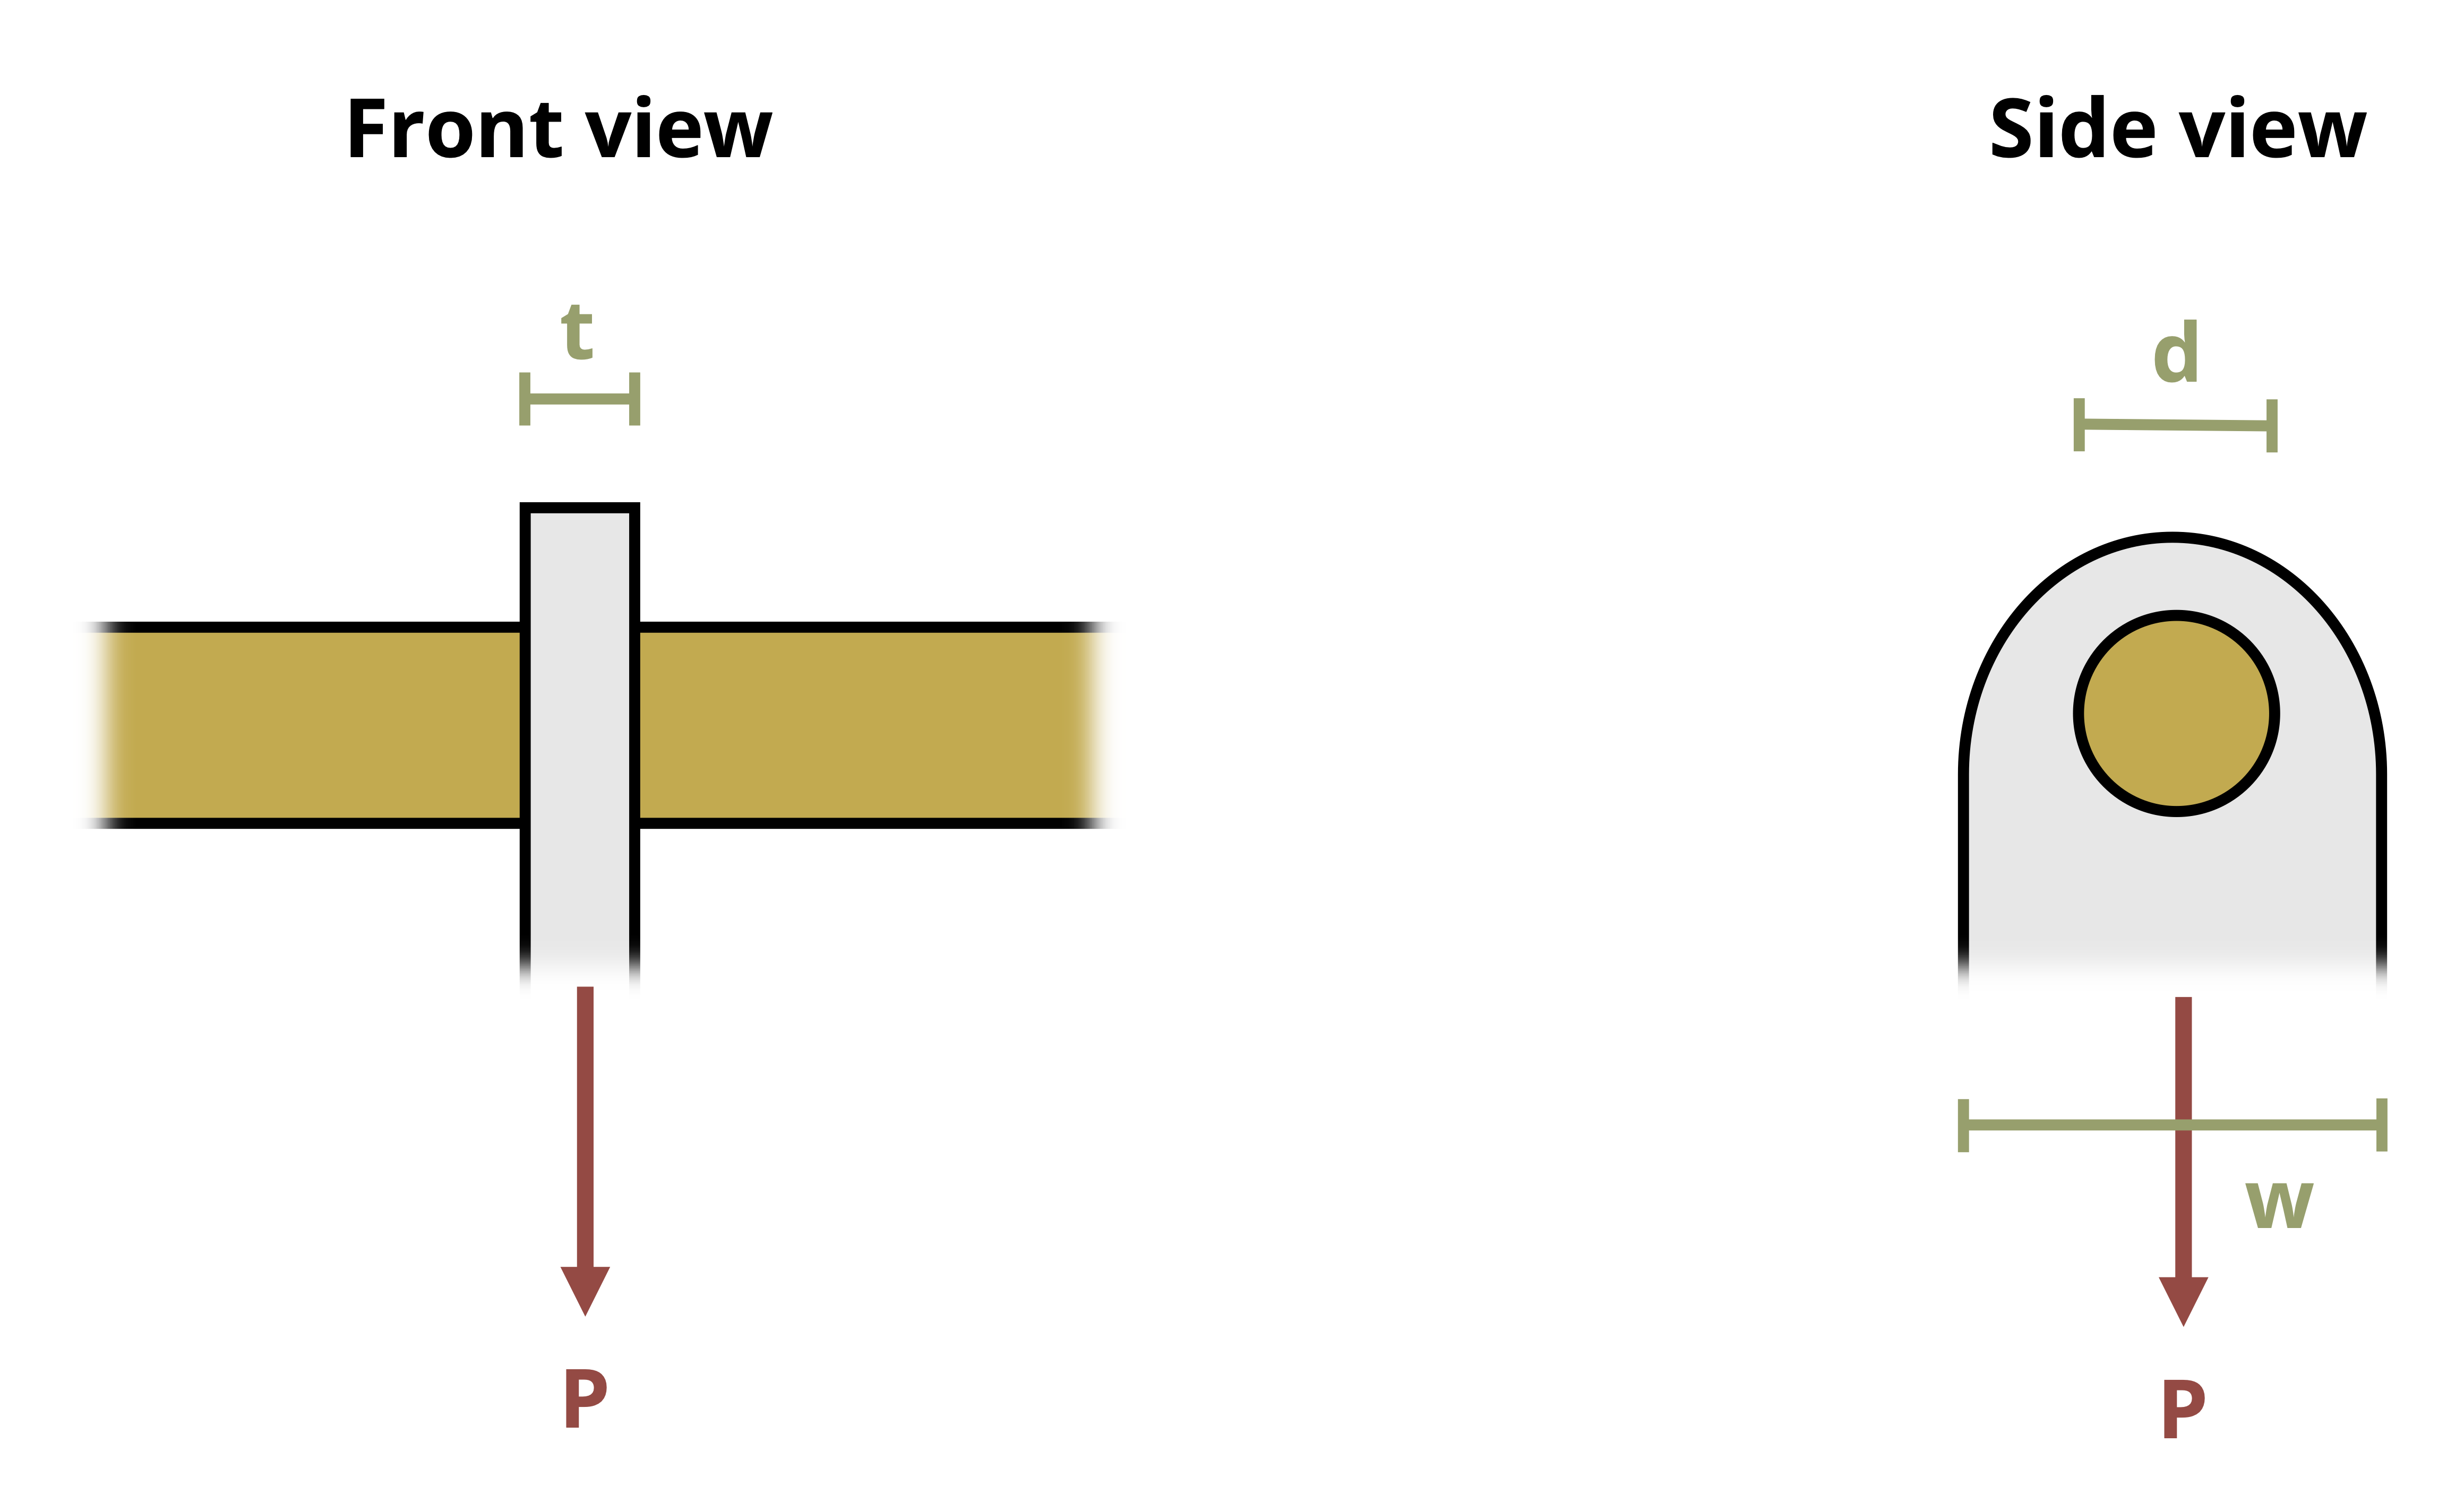
\includegraphics{images/169.png}

}

\caption{Figure 1: A steel connector plate is hung from a brass rod.}

\end{figure}%

\begin{Shaded}
\begin{Highlighting}[]
\NormalTok{\#| standalone: true}
\NormalTok{\#| viewerHeight: 600}
\NormalTok{\#| components: [viewer]}

\NormalTok{from shiny import App, render, ui, reactive}
\NormalTok{import random}
\NormalTok{import asyncio}
\NormalTok{import io}
\NormalTok{import math}
\NormalTok{from datetime import datetime}
\NormalTok{from pathlib import Path}

\NormalTok{problem\_ID="169"}
\NormalTok{d=reactive.Value("\_\_")}
\NormalTok{t=reactive.Value("\_\_")}
\NormalTok{W=reactive.Value("\_\_")}
\NormalTok{Fbrass = 70}
\NormalTok{Fsteel = 75}


\NormalTok{attempts=["Timestamp,Attempt,Answer,Feedback\textbackslash{}n"]}

\NormalTok{app\_ui = ui.page\_fluid(}
\NormalTok{    ui.markdown("**Please enter your ID number from your instructor and click to generate your problem**"),}
\NormalTok{    ui.input\_text("ID","", placeholder="Enter ID Number Here"),}
\NormalTok{    ui.input\_action\_button("generate\_problem", "Generate Problem", class\_="btn{-}primary"),}
\NormalTok{    ui.markdown("**Problem Statement**"),}
\NormalTok{    ui.output\_ui("ui\_problem\_statement"),}
\NormalTok{    ui.input\_text("answer","Your Answer in units of inches", placeholder="Please enter your answer"),}
\NormalTok{    ui.input\_action\_button("submit", "Submit Answer", class\_="btn{-}primary"),}
\NormalTok{    ui.download\_button("download", "Download File to Submit", class\_="btn{-}success"),}
\NormalTok{)}


\NormalTok{def server(input, output, session):}
\NormalTok{    @output}
\NormalTok{    @render.ui}
\NormalTok{    def ui\_problem\_statement():}
\NormalTok{        return[ui.markdown(f"A steel connector plate is hung from a brass rod of diameter \{d()\} = in. The plate has dimensions \{t()\} = in. and \{w()\} = in. Find the minimum load that will cause the connector or rod to fail. Assume the tensile and compressive failure stress for brass is 70 ksi and for steel is 75 ksi. Assume the shear failure stress for each material is one half of the tensile{-}compressive failure stress. ")]}
    
\NormalTok{    @reactive.Effect}
\NormalTok{    @reactive.event(input.generate\_problem)}
\NormalTok{    def randomize\_vars():}
\NormalTok{        random.seed(input.ID())}
\NormalTok{        d.set(random.randrange(0.8, 2, 0.1))}
\NormalTok{        t.set(random.randrange(0.3, 0.7, 0.1))}
\NormalTok{        w.set(d*2)}
        

\NormalTok{    @reactive.Effect}
\NormalTok{    @reactive.event(input.submit)}
\NormalTok{    def \_():}
        
\NormalTok{        instr= (Fsteel()/2)*(2*.866*d()/2)}
\NormalTok{        \#check=math.isclose(float(input.answer()),instr,rel\_tol=0.001)}
\NormalTok{        if math.isclose(float(input.answer()),instr,rel\_tol=0.001):}
\NormalTok{           check="*Correct*"}
\NormalTok{        else:}
\NormalTok{           check="*Not Correct.*"}
        
\NormalTok{        correct\_indicator = "JL" if check == "*Correct*" else "JG"}
        
\NormalTok{        feedback=ui.markdown(f"Your answer of \{input.answer()\} is \{check\}.  For reference in debugging this, the calculated instructor answer is \{instr\}")}
\NormalTok{        attempts.append(f"\{datetime.now()\}, \{input.submit()\},\{input.answer()\},\{check\}\textbackslash{}n")}
\NormalTok{        m=ui.modal(}
\NormalTok{          feedback,}
\NormalTok{          title="Feedback",}
\NormalTok{          easy\_close=True}
\NormalTok{        )}
\NormalTok{        ui.modal\_show(m)}
\NormalTok{    import random}
\NormalTok{    import string}

\NormalTok{def generate\_random\_letters(length):}
\NormalTok{    \# Generate a random string of letters of specified length}
\NormalTok{    return \textquotesingle{}\textquotesingle{}.join(random.choice(string.ascii\_lowercase) for \_ in range(length))   }

\NormalTok{random\_start = generate\_random\_letters(4)  }
\NormalTok{random\_end = generate\_random\_letters(4)    }

\NormalTok{encoded\_attempt = f"\{random\_start\}\{problem\_ID\}apoj\{len(attempts)+1\}\{correct\_indicator\}\{random\_end\}\{input.ID()\}"}


\NormalTok{attempts.append(f"\{datetime.now()\}, \{encoded\_attempt\}\textbackslash{}n")}

\NormalTok{    @session.download(}
\NormalTok{        filename=lambda: f"Problem\_Log{-}\{problem\_ID\}{-}\{input.ID()\}.csv"}
\NormalTok{    )}
\NormalTok{    async def download():}
\NormalTok{        \# This version uses a function to generate the filename. It also yields data}
\NormalTok{        \# multiple times.}
\NormalTok{        yield "Timestamp,Encoded Attempt\textbackslash{}n"}
   
\NormalTok{        for attempt in attempts:}
\NormalTok{          await asyncio.sleep(0.25) }
\NormalTok{          yield attempt}

\NormalTok{app = App(app\_ui, server)}
\end{Highlighting}
\end{Shaded}




\end{document}
